\documentclass[11pt, norsk]{article}
%\usepackage[latin1]{inputenc}
\usepackage[T1]{fontenc}
\usepackage[utf8]{inputenc}
\usepackage[norsk]{babel}   % S P R A A K
\usepackage{mathpazo}
\usepackage{euler}

% \usepackage{graphicx}    % postscript graphics
\usepackage{amssymb, amsmath, amsthm, amssymb} % symboler, osv
\usepackage{mathrsfs}
\usepackage{url}
\usepackage{thmtools}
\usepackage{enumerate}  % lister $  
\usepackage{float}
\usepackage{tikz}
\usetikzlibrary{calc}
\usepackage{tikz-3dplot}
\usepackage{subcaption}
\usepackage[all]{xy}   % for comm.diagram
\usepackage{wrapfig} % for float right
\usepackage{hyperref}
\usepackage{mystyle} % stilfilen      

%&\usepackage[a5paper,margin=0.5in]{geometry}

\begin{document}
\title{Notater til tredjesemestersrapportering}
\author{Fredrik Meyer}
\maketitle 

\section{Begreper}

Gitt et simplisialkompleks $\K$ kan vi lage et ideal i polynomringen med like mange variabler som $\K$ har hjørner. Idealet $I_\K$ er da definert til å være generert av monomer med eksponenter som svarer til \emph{ikke-fasetter} i $\K$.

La eksempelvis $\K$ være en firkant med hjørner $x_1,x_2,x_3,x_4$. Da er $\I_\K$ generert av $x_1x_3$ og $x_2x_4$.

Et monomideal er alltid gradert, så vi kan lage $\PP(\K) := \Proj (P/I_\K)$, som er et projektivt skjema utstyrt med en ampel linjebunt $\OO(1)$. Det kan vises at $H^i(\PP(\K), \OO_{\PP(\K)}) \simeq H^i(\K,k)$, hvor venstresiden er knippekohomologi og høyresiden er simplisialkohomologi.

Dermed vil enhver deformasjon av $\K$ ha samme kohomologi som den topologiske realisasjonen til $\K$. Hvis for eksempel $\K$ er en sfære, og $\PP(\K)$ er glattbar, så vil glattingen være Calabi-Yau, etc.

Deformasjonsteorien til Stanley-Reisner-skjemaer er godt beskrevet. Se for eksempel \cite{deforming_christophersen}.

\section{Hva jeg jobber med i dag}

La $D$ være en sekskant. La $\K$ være simplisialkomplekset $D \ast D$, altså simplisialkomplekset som har maksimale fasetter $(f_1,f_2)$ hvor $f_1,f_2$ er kanter i sekskanten. Da er $\K$ en tredimensjonal sfære med $f$-vektor $(1, 12, 48, 72, 36)$. 

Dette gir oss et Stanley-Reisner-ideal $I_\K$ med $18$ generatorer. Vi har $I_K=I_{D_1} + I_{D_2} \subseteq k[x_1,\cdots,x_{12}]$.

La $\K'$ betegne $\K \ast \{v\}$, suspensjonen av $\K$. Dette er et nytt simplisialkompleks med et ekstra hjørne, og svarer til kjegla over en $3$-sfære. Man kan forestille seg dette som en $4$-dimensjonal ball med $v$ som eneste indre punkt, og $\K$ som randa $\approx S^3$.

La $dP$ være polytopet avbildet i Figur 1 og la $P=dP \times dP$ være produktet. Da får vi et polytop med $36$ hjørner og f-vektor som er omvendt av $f$-vektoren til $\K$. Det følger da at $P^\circ$, det polare polytopet, har samme $f$-vektor som $\K$, og faktisk viser det seg at $\K$ er abstrakt isomorf med en triangulering av randa til $P^\circ$.

\begin{figure}
\label{fig:hexagon}
\centering
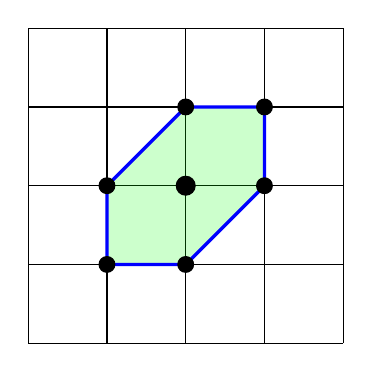
\begin{tikzpicture}
  \draw (0, 0) grid (4, 4);  
\draw [very thick, color=blue, fill=green, fill opacity=0.2]
(1,1) -- (2,1) -- (3,2) -- (3,3) -- (2,3) -- (1,2) -- cycle;
\draw [fill=black]  (1, 1) circle (0.1);
\draw [fill=black]  (2, 1) circle (0.1);
\draw [fill=black]  (3, 2) circle (0.1);
\draw [fill=black]  (3, 3) circle (0.1);
\draw [fill=black]  (2, 3) circle (0.1);
\draw [fill=black]  (1, 2) circle (0.1);
\draw [fill=black]  (2, 2) circle (0.12);
\end{tikzpicture}
\caption{Et heksagon.}
\end{figure}

Det følger da fra standard teoremer at det finnes en flat deformasjon av $\PP(\K')$ til den toriske varieteten $X_{P^\circ}$ (som beskrevet i \cite{sturmfels}. Siden $\PP(\K)$ er et komplett snitt (hyperflate!) i $\PP(\K')$, følger det at vi får en flat deformasjon av $\PP(\K)$ til en hyperflate i den toriske varieteten $X_{P^\circ}$.

Denne hyperflaten er dermed en $3$-dimensjonal projektiv varietet $Y$ med trivielt kanonisk knippe, og med en mild definisjon av Calabi-Yau er dette en Calabi-Yau-varietet. Vi kan så gjøre en såkalt ``MPCP-resolusjon'' (\emph{``maximal projective crepant partial resolution''}) av $X_{P^\circ}$, og få en glatt Calabi-Yau $\widetilde Y$ hvis Hodge-tall kan beregnes på en datamaskin (oppskriften er å telle gitterpunkter i fasetter til $P^\circ$).

\begin{prop}
Stanley-Reisner-skjemaet $\PP(\K)$ deformerer til en singulær Calabi-Yau $Y$ som har en krepant resolusjon $\widetilde Y$ hvis Hodge-tall er $h^{11}=44$ og $h^{12}=8$. Dermed er Euler-karakteristikken $\chi=72$.
\end{prop}

Det er også mulig å beskrive singularitetene til $Y$.

\begin{prop}
$Y$ har $48$ isolerte singulariteter, hvorav $36$ er $3$-dimensjonale noder (lokalt $xy-zw=0$), og $12$ er kjegler over sekskanter.
\end{prop}

Dette gir oss med en gang hva $H^0(Y,\mathcal T^1_{Y/k})$ er. Nodene har $T^1=1$, mens kjeglene over sekskantene har $T^1=3$. Dermed har vi at $\dim_k H^0(Y,\mathcal T^1_{Y/k})$ er $72$. Dette er derimot ikke hele modulen av infinetesimale deformasjoner siden vi også kan ha bidrag fra $H^1(Y,\Theta_Y)$, men denne er vanskelig å beregne for singulære $Y$.

Så snart du har en Calabi-Yau-mangfoldighet er det interessant å gjøre speilsymmetri. Problemet er da å finne et ``speil'' $Y^\circ$ med speilede Hodge-tall. For toriske varieteter finnes det en standard måte å gjøre dette på (Batyrev-konstruksjonen), men det finnes andre, mer hypotetiske konstruksjoner.

Én er såkalte ``extremal transitions'': start med en glatt Calabi-Yau-varietet, og degenerer denne til en singulær varietet med ikke altfor gærne singulariteter. Gjør så en resolusjon av singulariteter, og få en ny glatt Calabi-Yau-varietet. Det viser at denne konstruksjonen ofte gir opphav til speilede varieteter (altså at Hodge-tallene $h^{ij}(Y)=h^{ji}(Y^\circ)$). 

Vi står igjen med flere spørsmål som jeg jobber med å svare på:
\begin{enumerate}
\item Finnes faktisk en glatting av $Y$? Hvis så, hva er Hodge-tallene?
\item Stemmer denne glattingen overens med speilet spådd av Batyrev-konstruksjonen? 
\item Speilsymmetri er relatert til kurvetelling på Calabi-Yau-ene, og dette er relatert til å løse noen differensiallikninger definert ved potensrekker. Disse kan løses for å teste speilsymmetriforutsigelsene. 
\end{enumerate}

Det gjenstår mye arbeid, og veldig mye tid har blitt brukt på å lære meg ting som torisk geometri, begreper i speilsymmetri, og generelt lære meg algebraisk geometri-resultater.

\bibliographystyle{plain}
\bibliography{bibliografi}

\end{document}
